\chapter{Příklady návrhu virtualizace síťových funkcí}

V této kapitole bude uvedeno několik příkladů, jak lze jednoduše vytvořit NFV v prostředí OpenStack a OpenContrail pomocí heat templatů. Všechna uvedená řešení byla testována v prostředí OpenStack s OpenContrailem, které bylo pro tyto účely poskytnuto společností tcp cloud a.s. 


\section{Architektura komponent}\label{sub:interaction}

\begin{figure}[h]
\begin{centering}
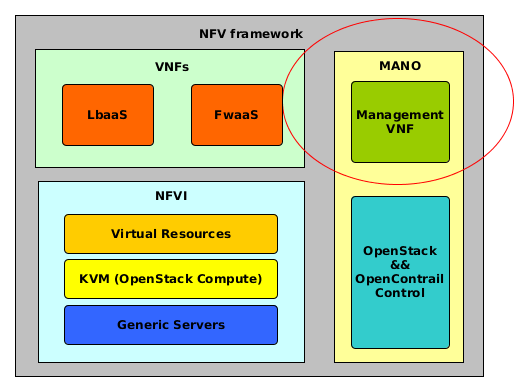
\includegraphics[scale=0.51]{images/VNF_overview}
\par\end{centering}
\caption{Architektura komponent\label{fig:VNF_overview}}
\end{figure}


\section{LbaaS}\label{sub:interaction}

Load-balancer as a Service má umožňovat uživatelům jednoduše 

\subsection{Neutron HAproxy}\label{sub:interaction}

Obrázek s virtuální topologii
Heat template + popis co v něm je

\section{FwaaS}\label{sub:interaction}

\subsection{PfSense}\label{sub:interaction}

PFSense je open-source firewall/router postavený nad operačním systémem FreeBSD.

\subsection{Fortigate VM}\label{sub:interaction}

Popis fortigate VM
Obrázek s topologii
Automatizace

